\documentclass[tikz,border=10pt]{standalone}
\usepackage{tikz}
\usetikzlibrary{shapes,arrows,positioning,fit,backgrounds}

\begin{document}
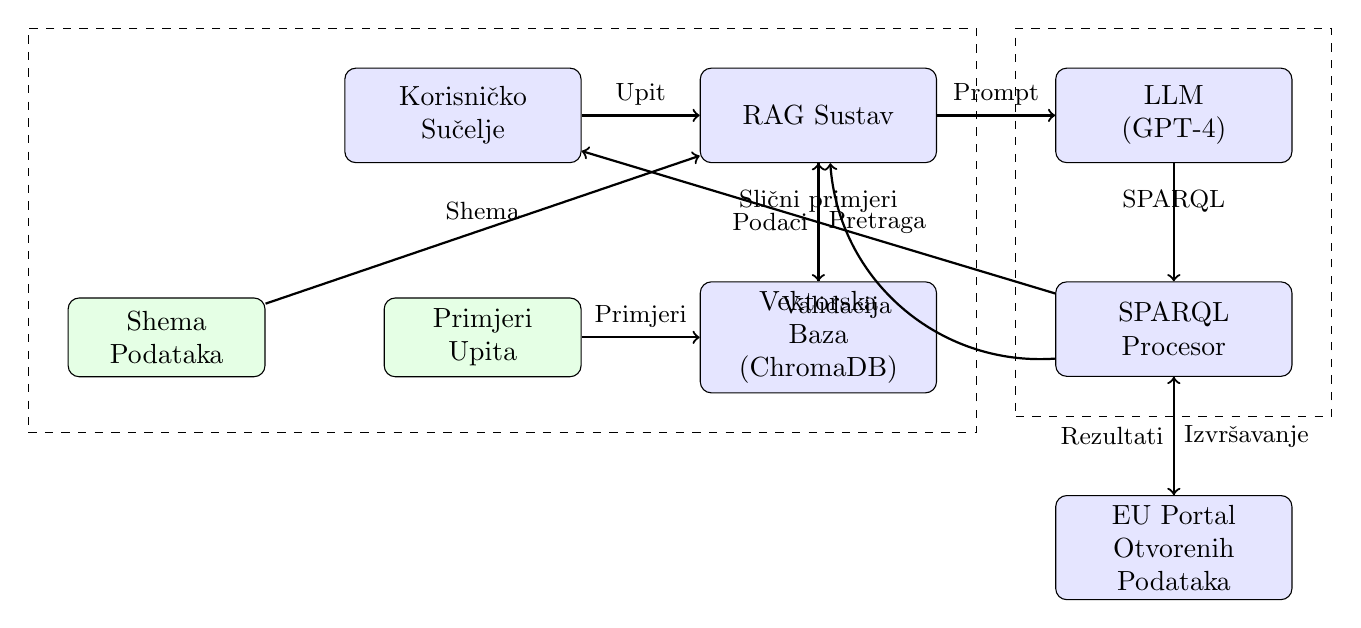
\begin{tikzpicture}[
    node distance=1.5cm,
    box/.style={rectangle, draw, rounded corners, minimum width=2.5cm, minimum height=1cm, align=center},
    component/.style={rectangle, draw, rounded corners, minimum width=3cm, minimum height=1.2cm, align=center, fill=blue!10},
    data/.style={rectangle, draw, rounded corners, minimum width=2.5cm, minimum height=1cm, align=center, fill=green!10},
    arrow/.style={->, thick},
    label/.style={font=\small}
]

% Main components
\node[component] (user) {Korisničko\\Sučelje};
\node[component, right=of user] (rag) {RAG Sustav};
\node[component, right=of rag] (llm) {LLM\\(GPT-4)};
\node[component, below=of rag] (vector) {Vektorska\\Baza\\(ChromaDB)};
\node[component, below=of llm] (sparql) {SPARQL\\Procesor};
\node[component, below=of sparql] (euportal) {EU Portal\\Otvorenih\\Podataka};

% Data stores
\node[data, left=of vector] (examples) {Primjeri\\Upita};
\node[data, left=of examples] (schema) {Shema\\Podataka};

% Background boxes
\begin{scope}[on background layer]
    \node[fit=(rag)(vector)(examples)(schema), draw, dashed, inner sep=0.5cm, label=above:Obrada] {};
    \node[fit=(llm)(sparql), draw, dashed, inner sep=0.5cm, label=above:Generiranje] {};
\end{scope}

% Arrows
\draw[arrow] (user) -- node[label, above] {Upit} (rag);
\draw[arrow] (rag) -- node[label, above] {Prompt} (llm);
\draw[arrow] (llm) -- node[label, above] {SPARQL} (sparql);
\draw[arrow] (sparql) -- node[label, right] {Izvršavanje} (euportal);
\draw[arrow] (euportal) -- node[label, left] {Rezultati} (sparql);
\draw[arrow] (sparql) -- node[label, left] {Podaci} (user);

% Data flow arrows
\draw[arrow] (rag) -- node[label, right] {Pretraga} (vector);
\draw[arrow] (vector) -- node[label, above] {Slični primjeri} (rag);
\draw[arrow] (examples) -- node[label, above] {Primjeri} (vector);
\draw[arrow] (schema) -- node[label, above] {Shema} (rag);

% Feedback loop
\draw[arrow, bend left=45] (sparql) to node[label, left] {Validacija} (rag);

\end{tikzpicture}
\end{document}